\chapter{Introduction}
\label{chap:1}




\section{Motivation}

\noindent Originally, the ledger is the foundation of accounting. However, it is not difficult to find that there are many shortcomings in the long-term use of traditional ledgers. For example, low efficiency, high cost, opacity and easy to cause fraud and abuse issues.\\

\noindent With the development of information technology, these ledgers have gradually evolved into digital technology. Distributed ledger is a major leap after the digitization of ledger-based technology. A distributed ledger is a database that is shared, replicated, and synchronized between network members\cite{brakeville2016blockchain}. It records transactions between network participants, such as the exchange of assets or data. From a technical point of view, the Distributed Ledger Technology (DLT) not only inherits the traditional bookkeeping philosophy but also has its unique innovations, which have some advantages that traditional ledgers cannot reach.\\

\noindent Based on the background above, there exist many distributed ledgers and for them to be fully distributed they need to communicate with each other and also traditional ledgers. Otherwise, the consistency between the ledgers of different entities across the chain would not be guaranteed. There have been many different approaches such as cross-chain protocols and platforms released to realize the cross-chain transactions, so it is worthy to find out the differences between them.


\section{Research Objectives/Research Questions, Research Methodology}

\noindent There is one technical issue that affects the blockchain developers, that is the communication. A single blockchain network is a relatively closed system that does not actively interact with the outside world. The assets of each chain are also an independent value system. If we can break through the interoperability among different ledgers and let the value circulate in the wider world, it will inevitably promote the rapid development of the blockchain industry. Cross-chain technology is dedicated to building a bridge of trust between ledgers, breaking the situation of an isolated value system, and realizing asset interoperability in order to achieve a true win-win situation.\\

\noindent This project makes uses of qualitative research strategy, where the research approach always implemented as interpretivism. To gain a standard requirement/need for cross-ledger communication model, the variety of factors are governed by all valuable findings through the research, which is not easily quantifiable (measurable). Therefore qualitative approach was found to be most applicable for this study.\\

\noindent For the purpose of this research, I decided to use literature review first to gain a deep understanding of cross-ledger history and realization of communications through published papers. Then the key point is the case study among popular projects. By studying the different cross-chain implementations, exacting the main idea of them, we can summarize and categorize them into different groups. Hence, identify patterns and commonalities in the cross-chain field. Even help more and more developers to consummate the blockchain design.


\section{Research Contributions}

\noindent My research has contributed to the universal demanding and requirements on cross-ledger communication towards blockchain areas. In particular, I have focused on the problems that the realization of cross-chain communication is facing.\\

\noindent For a long time since Bitcoin open the blockchain era, the blockchain world is like the single-machine time back in the 1960s. Every blockchain is highly independent and difficult to communicate with each other. Hence, the data and services in the blockchain world are confined to the individual blockchain, as a result, this phenomenon will discourage development. As if we could find a standardized cross-chain protocol/platform that could link all blockchain systems, and the services could be more specific and complete due to the co-operate of blockchains. The popularization and mature of cross-chain technology will lead a revolutionary development in the blockchain field. And different from the Internet to achieve the circulation of information, cross-ledger could realize the circulation of value.\\

\noindent To understand different patterns or implementations of cross-chain technology, we need to start with the history of cross-chain and grasp the main idea of chain interoperability based on literature review. Based on those findings, we could summarize the key problems the blockchains now facing, according to those difficulties I will give several examples through the case study in the following paragraph. This is where my research contributes significantly to the existing literature. The comparison from various aspects will next lead to a standard and universal needs of the cross-chain area. In my thesis, I have considered the following three major aspects of this study as shown in Figure \ref{fig:contri}

    
    \begin{figure}[H]
    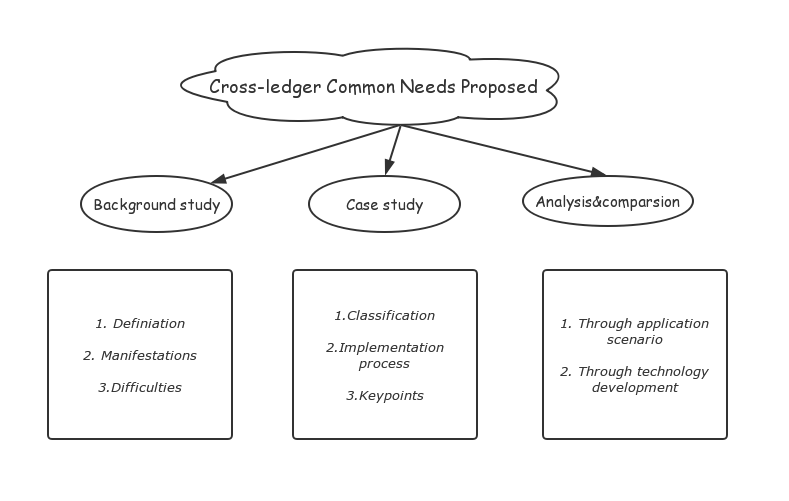
\includegraphics[width=1\textwidth]{./figures/contri.png}
    \centering
    \caption{Research components of cross-chain communication}%\protect\footnotemark}
    \centering
    \label{fig:contri}
    \end{figure}
    
\section{Thesis Organization}

This thesis is organized into five chapters as follows:

$\bullet $ Chapter \ref{chap:1} concentrates on the research value and market meaning of this thesis, then briefly introduces the concept of cross-chain communication.

$\bullet $ Chapter \ref{chap:2} studies the background of the cross-chain project by classifying different manifestations of cross-chain communication as well as pointing out the problems cross-ledger communication facing.

$\bullet $ Chapter \ref{chap:3} focuses on the theoretical solutions that will address the difficulties, discusses the communication process of various cross-chain projects based on different group rules. 

$\bullet $ Chapter \ref{chap:4} put efforts on analyze the market demand situation and discuss the applications that could be adopted, compare the technology development of some representative projects.

$\bullet $ Chapter \ref{chap:5} summarizes the findings during the research and suggests several ideas for related future work.

$\bullet $ \nameref{app:A} contains a comparison table that evaluating 20 cross-chain projects from several valuable aspects.

$\bullet $ \nameref{app:B} lists implementation code pieces with essential functions explained and the utilization of smart contracts, for further test use.
  